\documentclass[parskip=full,11pt]{scrartcl}
%\usepackage{pdfpages}
\usepackage[utf8]{inputenc}
\usepackage{amssymb}
\usepackage[T1]{fontenc}
\usepackage[german]{babel}
\usepackage[yyyymmdd]{datetime} 
\usepackage{hyperref}
\usepackage[toc, nonumberlist, automake]{glossaries} %added automake option
\usepackage{csquotes}
\usepackage{graphicx}
\hypersetup{
 		pdftitle={Entwurf},
 		bookmarks=true,
 }
\usepackage{fancyhdr}%<-------------to control headers and footers
\usepackage[a4paper,margin=1in,footskip=.25in]{geometry}
\fancyhf{}
\fancyfoot[C]{\thepage} %<----to get page number below text
\pagestyle{fancy} %<-------the page style itself
 
\title{Entwurf}
\subtitle{Autorisierungsmanagement für eine virtuelle Forschungsumgebung für Geodaten}
\author{Alex\\Anastasia\\Atanas\\Dannie\\ Houra\\Sonya\\}
\date{11.01.18}
 % define custom lists
\usepackage{enumitem}

% add glossary
\makeglossaries
\newglossaryentry{GUI}
{
	name={GUI},
	description={Abk. GUI von englisch \textbf{G}raphical \textbf{U}ser \textbf{I}nterface,ist Grafische Benutzeroberfläche oder auch grafische Benutzerschnittstelle, über die eine Person eine Software kontrollieren kann.  Im Idealfall ist sie benutzerfreundlich, so dass die Interaktion auf natürliche und intuitive Weise geschehen kannIm Idealfall ist sie benutzerfreundlich, so dass die Interaktion auf natürliche und intuitive Weise geschehen kann}, 
}
\newglossaryentry{ORM}
{
	name={ORM},
	description={Abk. ORM von englisch \textbf{O}bject-\textbf{R}elational \textbf{M}apping, ist eine Programmiertechnik zum Konvertieren von Daten zwischen inkompatiblen Systemen mit objektorientierten Programmiersprachen. Dies erzeugt in Wirklichkeit eine "virtuelle Objektdatenbank", die innerhalb der Programmiersprache verwendet werden kann}, 
}
\newglossaryentry{HTML}
{
	name={HTML},
	description={Abk. HTML von englisch \textbf{H}yper\textbf{t}ext \textbf{M}arkup \textbf{L}anguage, Auf Deutsch bedeutet dies  „Auszeichnungssprache für verknüpften Text“. Er ist Voraussetzung für die Programmierung und das Design von Webinhalten. Andere Standards wie PHP bauen in erheblichem Maße auf HTML auf }, 
}
\newglossaryentry{URL}
{
	name={URL},
	description={Abk. URL von englisch \textbf{U}niform \textbf{R}esource \textbf{L}ocator, wird häufig als Webadresse bezeichnet. Diese Adresse wird verwendet, um eine im Web vorhandene Ressource durch eine ASCII-Zeichenfolge zu bezeichnen. Ressourcen können variiert werden (Webseite, Video, Ton, Bild, Animation, E-Mail-Adresse ...)}, 
}
\newglossaryentry{Geheimnisprinzip}
{
	name={Geheimnisprinzip},
	description={Vom Innenleben einer Klasse soll der Verwender – gemeint sind sowohl die Algorithmen, die mit der Klasse arbeiten, als auch der Programmierer, der diese entwickelt – möglichst wenig wissen müssen },
}


\usepackage{linegoal,listings}
\newsavebox{\mylisting}
\makeatletter
\newcommand{\lstInline}[2][,]{%
	\begingroup%
	\lstset{#1}% Set any keys locally
	\begin{lrbox}{\mylisting}\lstinline!#2!\end{lrbox}% Store listing in \mylisting
	\setlength{\@tempdima}{\linegoal}% Space left on line.
	\ifdim\wd\mylisting>\@tempdima\hfill\\\fi% Insert line break
	\lstinline!#2!% Reset listing
	\endgroup%
}
\makeatother
\setlength{\parindent}{0pt}% Just for this example

\lstset{basicstyle=\footnotesize\ttfamily,breaklines=true}
\lstset{framextopmargin=50pt,frame=bottomline,showstringspaces=false,upquote=true}


\RedeclareSectionCommand[style=section,indent=0pt,font=\usekomafont{partnumber}]{part}
\renewcommand*{\partformat}{\thepart\enskip}

\RedeclareSectionCommand[beforeskip=0pt ,afterskip=0pt]{subparagraph}



\newcommand{\class}[1]{\subsubsection*{\lstinline[basicstyle=\ttfamily\large]{#1}}}

% command for an attribute
\newcommand{\atr}[4]{\lstinline{[#3]} \textbf{\lstinline{#1 : #2}} \newline #4}

% command for a method
\newcommand{\mtd}[5]{\lstinline{[#4]} \textbf{\lstinline{#1(#3) : #2}} \newline #5}

% command for a constructor
\newcommand{\ctr}[4]{\lstinline{[#3]} \textbf{\lstinline{#1(#2)}} \newline #4}
%command for formating an inline source code
\newcommand{\inlinecode}[1]{\lstInline[breaklines=true]{#1}}

% make the bullet symbol in lists a circle for level 2
\renewcommand{\labelitemii}{$\circ$}




 
\begin{document}
 
 \begin{titlepage}
 	
 	\begin{center}
 	
\includegraphics[width=0.5\linewidth]{res/KITLogo.png}\\
 	\vspace{2cm}
 	{\scshape\LARGE\bfseries Entwurf \par}
 	\vspace{0.5cm}
 	{\scshape\Large Praxis der Softwareentwicklung\\}
 	\vspace{1cm}
 	{\scshape\Large Wintersemester 17/18\\}
 	\vspace{2cm}
 	{\huge\bfseries Autorisierungsmanagement für eine virtuelle Forschungsumgebung für Geodaten\par}
 	\vspace{2cm}
 	\vfill
 	{\bfseries {\Large Autoren}:\par}
 	{\Large Bachvarov, Aleksandar }\\
 	{\Large Dimitrov, Atanas }\\
 	{\Large Mortazavi Moshkenan, Houraalsadat }\\
 	{\Large Sakly, Khalil }\\
 	{\Large Slobodyanik, Anastasia }\\
 	{\Large Voneva, Sonya}\\
 	\vfill
 	{\large 11.01.18 \par}
 	\end{center}
 \end{titlepage}
 
 \tableofcontents
 
 \newpage
 \section{Einleitung}
 
Während der Entwurfsphase wurde das Konzept für das zu erstellende Produkt formuliert. Die in diesem Dokument definierte Softwarearchitektur legt die Struktur und das Verhalten des Produkts fest. Durch Bestimmung grundlegender Entwurfsentscheidungen haben sich einige sinnvolle Änderungen zum Pflichtenheft ergeben. \\
Für die Funktion „Benutzer suchen“ wurden Suchparameter erweitert: die Suche soll anhand von Name, Email sowie Domain des Benutzers möglich sein. 
Nach dem Löschen einer Ressource werden alle Benutzer, die Besitzerrechte für diese Ressource hatten, benachrichtigt. 
Als Ressourcendaten werden auch Typ und kurze Beschreibung der Ressourcen gespeichert. 
Administratoren des Portals sollen in der Lage sein andere Benutzer zu blockieren.

 
 \section{Architektur}
 
 \subsection{Model View Template (MVT)} \label{MVT}
Beim Design des Autorisierungsmanagement Web-Portal wird schnell deutlich, dass eine strikte Trennung
zwischen Datenbank, Applikationslogik (Code) und Benutzeroberfläche (view) von Vorteil ist. Das Model-View-Template Prinzip (MVT),Das in Abbildung 1 gezeichnet ist, realisiert diese Trennung und wird in der Webanwendung eingesetzt.\\
Das Model-View-Template ist eine Ableitung des Architektur-Pattern-View-Presenter (MVP) -Musters und wird hauptsächlich zum Erstellen von Benutzerschnittstellen verwendet.\\
 
 
 \begin{figure}[ht!]
 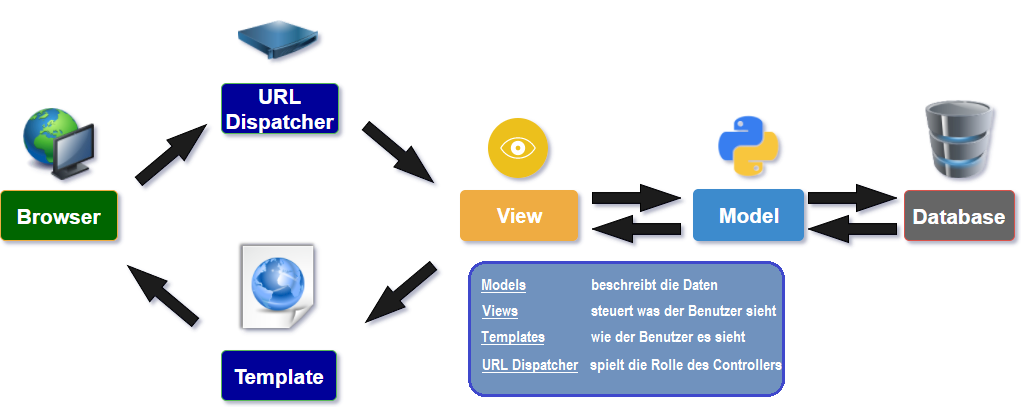
\includegraphics[width=1.1\textwidth]{res/MVTdiagramm.png}
  	 	\centering
  	    \caption{MVT Architektur}
 \end{figure}
  \newpage


 	\textbf{•} Der \textbf{URL-Dispatcher} \emph{(urls.py)} ordnet die angeforderte \gls{URL} einer \textbf{View-Funktion} zu und ruft sie auf.\\
 	\textbf{•} Die \textbf{View-Funktion} \emph{(views.py)} führt die angeforderte Aktion aus, bei der normalerweise in die Datenbank gelesen oder geschrieben wird. es kann auch andere Aufgaben beinhalten.\\
 	\textbf{•} Das \textbf{Model} \emph{(models.py)} definiert die Daten in Python und interagiert damit. Dies ist normalerweise in einer relationalen Datenbank \emph{(SQLite)} enthalten.\\
 	\textbf{•} Nach der Ausführung der angeforderten Aufgaben gibt die \textbf{View} ein HTTP-Antwortobjekt an den Webbrowser zurück, normalerweise nach dem Übergeben der Daten durch ein \textbf{Template}.\\
 	\textbf{•} \textbf{Template} gibt normalerweise \gls{HTML}-Seiten zurück. Die Django-Template-sprache bietet HTML-Autoren eine einfach zu erlernende Syntax und bietet gleichzeitig die gesamte für die Präsentationslogik erforderliche Leistung. \\
 	

 \subsection{Betrieb des Django ORM} 
 
Das \gls{ORM} Django ist ein in Python geschriebenes quelloffenes Webframework, das Beispielweise folgendermaßen funktioniert :\\
 • Erstellt Django SQL-Tabellen aus der Modellen (klassen) mit alle klassen-Attributen als Tabellenspalten, z.b SQL-Tabelle 'Request' aus dem Modell 'Request'. All dies geschieht wiederum ohne eine SQL-Abfrage zu schreiben.\\
 • Um die Tabellen auszufüllen wird die Methode save() benutzt.\\
 • Auf die gleiche Weise ist es möglich, alle Einträge der Tabelle zu erhalten ,Daher werden Instanzen von dem gewünschten Objekt zurückgegeben, einen für jeden Eintrag in der Tabelle, ein Beispiel für alle Request-Objekte zu haben wird in der Abbildung 2 gezeigt:\\

  	\vspace{2cm}



\begin{figure}[ht!]
  	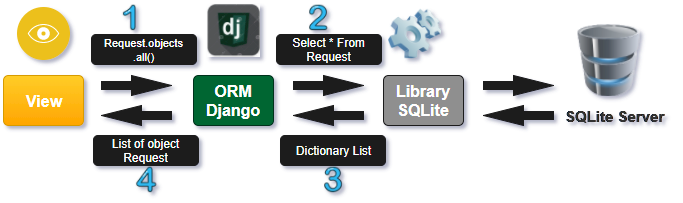
\includegraphics[width=1.05\textwidth]{res/MVTpart2.png}
  	 	\centering
  	    \caption{MVT mit Django}
 \end{figure}

 	

\newpage
 \subsection{Paketenstruktur}
 Das folgende \hyperref[packages]{Paketendiagramm} stellt die verschiedenen Paketen, die in der Entwurfsphase gestaltet werden(inkl. Paketen die von Django vordefiniert sind - ``Extern``), und ihre Beziehungen zueinander dar. Den Inhalt dieser Paketen wird im Abschnitt ``Paketenübersicht`` beschrieben.\\
 %beschreibung der beziehungen kommen bald
 \begin{figure}[h]
 	\includegraphics[width = 1.0\textwidth]{res/packages}
 	\centering
 	\caption{Paketendiaramm}
 	\label{packages}
 \end{figure}
 

 \subsection{Entwurfsmuster}
 Bei diesem Entwurf werden Entwurfsmuster verwendet, um einzelne Komponenten voneinander zu entkoppeln und das \gls{Geheimnisprinzip} zu unterstützen. 
 \subsubsection*{Strategie-Muster}
 \begin{figure}[ht!]
 	\centering
 	\includegraphics[width=\textwidth]{res/strategie.png}
 	\caption{Sterategie-Muster}
 \end{figure}
 Das Strategy-Muster kommt in den Klassen ``\textit{Reauest}``, ``\textit{AccessRequest}`` und ``\textit{DeletionRequest}`` bei der Funktion ``\textit{accept()}`` zum Einsatz. Dieses Muster hat das Ziel, eine Familie von Algorithmen zu definieren, zu kapseln und austauschbar zu machen.
 
 \subsubsection*{Befehlsmuster}
 \begin{figure}[ht!]
 	\centering
 	\includegraphics[width=0.85\textwidth]{res/Befehl.png}
 	\caption{Befehlsmuster}
 	\label{Befehl}
 \end{figure}

 Das Befehlsmuster ist zur Bearbeitung von den Requests (Funktionen ``\textit{deny()}`` und ``\textit{accept()}`` in Klasse ``\textit{Request}``) verwendet.Mit Hilfe dieses Musters wird die Bearbeitung der Requests von den Requests selbst, wie in der   \hyperref[Befehl]{Abbildung 5} angezeigt ist, getrennt.\\
 Das Befehlsmusters ermöglicht es, ein bestimmtes Ereignis in einem dafür vorgesehenen Handler
 zu bearbeiten und dieses damit in einem Objekt zu kapseln. Jeder Handler lässt sich eindeutig einer Aufgabe
 und einem Ereignis zuordnen, sodass keine Verschränkung zwischen zwei verschiedenen Handlern auftritt.
 Außerdem lässt sich leichter ein weiterer Handler hinzufügen oder ein bestehender Handler austauschen.
 
 \subsubsection*{Bequemlichkeitsmethode-Muster}
 Das Bequemlichkeitsmethode-Muster ist in der Klasse ``\textit{Owner}``
 bei den Funktionen ``\textit{allowAccessPermission(reqestID)}`` und ``\textit{allowAccessPermission(resourceID, userID)}`` verwendet. Dieses Muster dient zum Vereinfachen des Funktionenaufrufs durch die Bereitstellung häufig
genutzter Parameterkombinationen in zusätzlichen Funktionen
(Überladen).
  \subsection{URL Verzeichnis}
Alle Interaktionen zwischen den Benutzern und dem Produkt werden durch eine graphische Benutzeroberfläche (GUI) unterstützt. Die \gls{GUI} des Produkts wird als eine Webseite dargestellt, wobei sämtlicher Inhalt und Funktionalität unter URL Verzeichnis abgelegt werden (\hyperref[URL Struktur]{\mbox{Abbildung 6}}). 

\begin{figure}[ht!]
 	\centering
 	\includegraphics[width=\textwidth]{res/urls_Diagram.png}
 	\caption{URL Struktur des Portals. Jedes URL korrespondiert entsprechendem View. Schwarz beschriftete URLs weisen zu Views, die in Main-Fenster angezeigt werden, blaue - zu Dialogfenster. }
 	\label{URL-Struktur}
 \end{figure}
 
\textbf{pse-authoritation.com} – Mockup-Seite, dient zum Einloggen in das Portal, enthält Autorisierungsformular und wird nach der Entwicklung durch Autorisierungsmanagement des Systems, in welches das Projekt integriert wird, ersetzt. 
 
\renewcommand{\labelitemi}{$\bullet$}
\renewcommand{\labelitemii}{$\bullet$}
\renewcommand{\labelitemiii}{$\bullet$}
\begin{itemize}[itemsep=0pt]
\item \textbf{/profil} - Benutzerprofil-Seite, enthält persönliche Information des Benutzers und Übersicht der Requeste, die an den Benutzer adressiert sind.\\

Benutzerprofil-Seite ist mit Subseiten versehen:
\begin{itemize}[itemsep=0pt]
\item \textbf{/handle{\_}$<$requestID$>$} - Dialog für Bearbeitung des Requests, enthält ``Annehmen''- und ``Ablehnen``-Buttons, sowie ein Eingabefeld für kurze Begründung.
\item \textbf{/resources} - Seite mit Übersicht von Ressourcen, für die der Benutzer Besitzerrechte hat. Diese Seite enthält Subseiten:
\begin{itemize}[itemsep=0pt]
\item \textbf{/add{\_}new{\_}resource} - Seite für Erstellen neuer Ressourcen. Enthält Upload-Dialog, Dialog für Vergabe von Rechten und Eingabefelder für Namen und Beschreibung der Ressourcen.
\item \textbf{/$<$resourceID$>${\_}edit{\_}users{\_}permissions} - Seite für Vergabe und Entzug von Rechten für die Ressource.
\item \textbf{/$<$resourceID$>${\_}send{\_}deletion{\_}request} - Dialog für Absenden von Löschrequest für die Ressource.
\end{itemize}
\end{itemize}


\item \textbf{/manage{\_}users} - Administratorseite für Benutzerverwaltung, enthält Liste von Benutzern und Subseiten:
\begin{itemize}[itemsep=0pt]
\item \textbf{/block{\_}user} - Dialog zum Blockieren des Users.
\item \textbf{/delete{\_}user} - Dialog zum Löschen des Users.
\item \textbf{/$<$userID$>${\_}permissions{\_}for{\_}resources} - Dialog zur Änderung von Rechten des Benutzers.
\end{itemize}

\item \textbf{/manage{\_}resources} - Administratorseite für Ressourcenverwaltung, enthält Liste von Ressourcen und Subseiten:
\begin{itemize}[itemsep=0pt]
\item \textbf{/$<$resourceID$>${\_}permissions{\_}for{\_}users} - Dialog zur Änderung von Zugriffsrechten für die Ressource. 
\item \textbf{/delete{\_}resource} - Dialog zum Löschen der Ressource.
\end{itemize}
\item \textbf{/resources{\_}owerview} - Übersicht von Ressourcen, enthält Liste aller Ressourcen und folgende Subseiten:
\begin{itemize}[itemsep=0pt]
\item \textbf{/$<$resourceID$>${\_}info} - enthält Metadaten der Ressource.
\item \textbf{/$<$resourceID$>${\_}send{\_}request} - Dialog zum Absenden des Requests für die Ressource.
\end{itemize}
\item \textbf{/<resourceID>} - Ressourcenseite, enthält Metadaten und Link für Zugriff auf die Ressource.
\end{itemize} 

 
 \newpage
 \section{Datenhaltung}
 
Relevante Daten über die Benutzer, Ressourcen, deren Beziehungen (Rechte) und Interaktionen (Requests) werden in einer Datenbank gespeichert. Das in diesem Projekt benutzte Framework Django bietet integrierte  objektrelationale Abbildung für die Datenbanksysteme MySQL, Oracle, PostgreSQL und SQLite.\\
Da SQLite-Bibliotheken sich direkt in Anwendungen integrieren lassen, sodass keine weitere Server-Software benötigt wird, wurde entschieden, SQLite3-Syntax zu verwenden. Im Projekt wird das eingebettete Datenbanksystem (für Frontend nicht sichtbar) entworfen, sodass auf erweiterte Funktionalitäten von komplizierteren Datenbanksysteme verzichtet werden kann. Dabei entstehen auch einige Vorteile: die SQLite-Bibliothek ist nur wenige hundert Kilobyte groß und durch das Einbinden der Bibliothek wird die Anwendung um Datenbankfunktionen erweitert, ohne auf externe Softwarepakete angewiesen zu sein.
 \subsection{Datenbank}
 \begin{figure}[ht!]
 	\centering
 	\includegraphics[width=\textwidth]{res/database.png}
 	\caption{Datenbankschema}
 \end{figure}
 \newpage
 
    \begin{center}
    \textit{``A model is the single, definitive source of information about your data. It contains the essential fields and behaviors of the data you’re storing. Generally, each model maps to a single database table.``}
    \end{center}
    —Models | Django documentation\\\\
    
Die Tabelle ``User`` speichert einen eindeutigen Identifikator (\textit{ID}) des Benutzers, seinen Vor- und Nachnamen, sowie das Datum, an dem er sich registriert hat. Zusätzlich hat die Tabelle eine Spalte ``is\char`_admin``, die zur Unterscheidung zwischen ``normalem`` Benutzer und Administrator dient.\\
Metadaten über die Ressourcen werden in der Tabelle ``Resource`` gespeichert: ID, Name, generischer Typ, kurze Beschreibung und Erstellungsdatum. Zusätzlich hat jeder Eintrag in der Tabelle eine Link zur ``echten`` Resource.\\
In der Tabelle ``Request`` werden relevante Daten über die Requests gespeichert: ID, Erstellungsdatum, Typ des Requests (Zugriffs- oder Löschrequest), ID der Ressource, für die der Request gesendet wird und ID des Absenders. Die letzte zwei sind Foreign Keys aus den Tabellen ``Resource``, bzw. ``User`` (Pfeile 2 und 6). Auf diese Weise werden Redundanzen vermieden und die Datenbank bleibt konsistent. Requests werden sofort nach der Erstellung gespeichert und nach der Bearbeitung wieder gelöscht.\\
Abgesendete, noch nicht bearbeitete Requests werden in der Tabelle ``ReceivedRequest`` dupliziert, dabei wird ein Eintrag pro Empfänger erstellt. Diese Tabelle enthält folgende Spalten: ID und Typ des Requests und ID des Empfängers. ID des Requests und ID des Empfängers sind Schlüssel aus den Tabellen ``Request``, bzw. ``User`` (Pfeile 1 und 4).  Der Primary Key besteht aus dem Tupel $\{user{\_}ID, request{\_}ID, type\}$.\\
Rechte werden in der Tabelle ``Permission`` dargestellt. Jeder Eintrag dieser Tabelle präsentiert entweder Zugriffs- oder Besitzerrechte, dabei werden folgende Attribute gespeichert: ID des Benutzers, ID der Ressource und Typ des Eintrags (Zugriffs- oder Besitzerrechte). Die erste zwei sind Schlüssel aus den Tabellen ``User``, bzw. ``Resource`` (Pfeile 3 und 5). Alle Attribute zusammen formieren den Primary Key dieser Tabelle. \\
 
 \subsection{Logging}
 Mithilfe von einem externen Django Module (``Logging``) wird eine Log-Datei geführt. Diese Datei beinhaltet zeitlichgeordnete Ereignisse vom System. Informationen wie Senden eines Requests, Bearbeitung eines Requests, Erstellen/Löschen einer Ressource und Editieren von Rechten können der Log-Datei entnommen werden. Zu jedem Ereignis wird auch den genauen Zeitpunkt gespeichert.
 
 
 \section{Paketenübersicht}
 \subsection{Templates}
Da Django ein Web Framework ist, ist es notwendig HTML-Dateien dynamisch zu generieren. Ein typisches Konzept dafür ist der Einsatz von Vorlagen (Templates). Eine Vorlage beinhaltet statische Teile vom gewünschten HTML Output, sowie Syntax, die beschreibt wie dynamischen Inhalt eingefügt wird.
 \subsection{Static}
 Für die Webseite sollen zusätzliche Dateien wie Abbildungen, CSS- oder JavaScript-Dateien gespeichert werden. In Django sind diese Dateien als ``Static Files`` bezeichnet.
 \subsection{Model}
Ein Model enthält Informationen über die unerlässliche Felder und Verhalten von den Daten, die gespeichert sind.
Das Paket ``model`` besteht aus den Klassen ``User``, ``Owner``, ``Admin`` ``Resource``, ``Request``, ``AccessRequest`` und ``DeletionRequest``. Normalerweise wird jede Klasse zu einer Tabelle in der Datenbank übersetzt. Jedes Attribut einer Klasse wird dann eine Spalte in der entsprechenden Tabelle.
 \subsection{Views}
 View ist eine Funktion, die als Eingabe ein Web Request bekommt und gibt  eine Web Response aus. Diese Response kann prinzipiell alles beinhalten - zum Beispiel HTML Inhalt einer Webseite, ein Bild, eine 404 Error Seite, Weiterleitung zu anderer Webseite. Die View Funktion definiert was genau angezeigt wird, nachdem eine URL angefragt wird.\\
 Zum Paket ``views`` gehören alle Klassen, die eine solche Funktion spezifizieren.
 \subsubsection{Generic}
 Da bei der Entwicklung einer Webseite bestimmte Muster öfter vorkommen,  bietet Django eine Sammlung von solchen Views an. Diese Views haben eine abstrakte Form, damit sie mehrmals wiederverwendet werden können. Auf diese Weise spart man Zeit und Codezeilen.

 
 \subsection{Test}
 Dieses Paket beinhaltet zwei Unterpaketen - test{\_}models und test{\_}views entsprechend für die Model- und die Viewklassen. Jedes Unterpaket enthält eine Testklasse spezifisch für jede Model- oder Viewklasse. Jede Testklasse hat eine setUp() Methode, die die entsprechende Objekte zum Testen erstellt und eine oder mehrere Modultestsmethoden für jede öffentliche Methode der getesteten Klassen.
 
 \subsection{Extern}
 \subsubsection{Logging}
 Django bietet ein Logging Modul an, das von Python vordefiniert ist.
 Dieses Paket beinhaltet Klassen und Funktionen, die das Logging von Systemereignisse ermöglichen. 
 \subsubsection{EmailMessages}
 Wie bei der Logging Funktionalität, wird für das Senden von E-Mail-Benachrichtigungen auch ein externes Paket von Django verwendet. Die Struktur dieses Pakets wird während der Implementierungsphase klar sein. 
 
 
 \newpage
 \section{Klassenübersicht}
 \subsection{Model}
 \paragraph*{Klasse User}
 \class{User}
 User-Klasse bildet eine Elternklasse aller Benutzertypen. Sie stellt alle Attribute fest, die für Darstellung des Benutzers notwendig sind, und beschreibt Aktivitäten, die von allen Benutzertypen ausgeführt werden können.
\subparagraph*{Attribute} % skip this if there are no attribute
\begin{itemize}
	\item \atr{USER_ID}{String}{final} {Eindeutiger Identifikator des Benutzers}
	\item \atr{name}{String}{private}{Name und Vorname des Benutzers}	
	\item \atr{email}{String}{private}{Email des Benutzers}
\end{itemize}

\subparagraph*{Funktionen}  % skip this if there are no methods
\begin{itemize}
	\item \mtd{searchResource}{List<Resource>}{searchParameters: String} {public}{Funktion liefert  \inlinecode{List<Resource>}, die alle Ressourcen enthält, dessen Metadaten den \inlinecode{searchParameters} entsprechen.}
	
	\item \mtd{addResource}{Resource}{ }{public}{Funktion erstellt eine Instanz von Klasse \inlinecode{Resource}, Metadaten werden dabei in Datenbank gespeichert, wobei \inlinecode{User} als Besitzer dieser Ressource definiert wird}
	
	\item \mtd{accessResource}{void}{resourceID: String} {public}{Falls Instanz von der Klasse \inlinecode{User}, die diese Funktion aufruft, entsprechende Rechte hat, werden Metadaten der Ressource, deren \inlinecode{resourceID}} als Parameter übergeben wird, von Datenbank abgerufen.
	
	\item \mtd{sendAccessRequest}{void}{resourceID: String} {public}
	{An alle Besitzer der Ressource, deren \inlinecode{resourceID} als Parameter übergeben wird, wird /inlinecode{AccessRequest} gesendet.}
	
	\item \mtd{cancelRequest}{void}{requestID: String} {public}{Der Request, dessen \inlinecode{requestID}} als Parameter übergeben wird, wird aus der Datenbank gelöscht.
\end{itemize}

\newpage
  \paragraph*{Klasse Owner}
 \class{Owner extends User}
Diese Klasse erweitert Klasse \inlinecode{User}. Nachdem eine Instanz von \inlinecode{User} Klasse Besitzerrechte für eine oder mehrere Ressourcen bekommt, wird ein neuer Eintrag in der Datenbank-Tabelle ``Owner``, beziehungsweise eine neue Instanz von Klasse \inlinecode{Owner} erstellt. 
\paragraph*{Attribute} 

\subparagraph*{Funktionen}  % skip this if there are no methods
\begin{itemize}
	\item \mtd{allowAccessPermission}{void}{resourceID:String, userID:String}{public}{
	Instanz der Klasse \inlinecode{User} bekommt \inlinecode{AccessPermission} für Instanz der Klasse \inlinecode{Resource}. \inlinecode{userID} des Benutzers und \inlinecode{resourceID} der Ressource werden als Parameter übergeben. 
	}
	\item \mtd{allowAccessPermission}{void}{requestID:String}{public}{
	Diese Funktion ladet vorherige Funktion über, dabei wird als Parameter \inlinecode{requestID} eines Requests übergeben. Absender dieses Requests bekommt \inlinecode{AccesPermission} für die Ressource, deren  \inlinecode{Request.RESORCE_ID} gehört.
	}
	\item \mtd{deleteAccessPermission}{void}{resourceID:String, userID:String}{public}{
	Der Instanz der Klasse \inlinecode{User}, die übergebenes Parameter \inlinecode{userID} besitzt, wird \inlinecode{AccessPermission} für die Ressource, deren \inlinecode{resourceID} jeweil als Parameter übergeben wird, entzogen.
	}
	\item \mtd{denyAccessPermission}{void}{requestID:String}{public}{
	\inlinecode{AccessRequest} wird abgelehnt: Instanz, der \inlinecode{requestID} entspricht, wird gelöscht.
	}
	\item \mtd{allowOwnerPermission}{void}{resourceID:String, userID:String}{public}{
	Instanz der Klasse \inlinecode{User} bekommt \inlinecode{OwnerPermission} für Instanz der Klasse \inlinecode{Resource}. \inlinecode{userID} und \inlinecode{resourceID} diesen Instanzen werden als Parameter übergeben.
	}
	\item \mtd{sendDeletionRequest}{void}{resourceID:String}{public}{
	Diese Funktion erstellt eine Instanz der Klasse  \inlinecode{DeletionRequest}. Das übergebene Parameter \inlinecode{resourceID} wird als \inlinecode{Request.REQUEST_ID} und \inlinecode{userID} des \inlinecode{Owner} als \inlinecode{Request.SENDER_ID} gespeichert.
	}
\end{itemize}
\newpage
  \paragraph*{Klasse Admin}
 \class{Admin extends Owner}
 bla bla
 
\paragraph*{Attribute} % skip this if there are no attribute

\subparagraph*{Funktionen}  % skip this if there are no methods
\begin{itemize}
	\item \mtd{searchUser}{List<User>}{searchParameters:String}{public}{
	bla  \inlinecode{USER_ID}
	}
	
	\item \mtd{blockUser}{void}{userID:String}{public}{
	bla  \inlinecode{USER_ID}
	}
	\item \mtd{deleteUser}{void}{userID:String}{public}{
	bla  \inlinecode{USER_ID}
	}
	\item \mtd{deleteResource}{void}{resourceID:String}{public}{
	bla  \inlinecode{USER_ID}
	}
	\item \mtd{acceptDeletionRequest}{void}{requestID:String}{public}{
	bla  \inlinecode{USER_ID}
	}
	\item \mtd{denyDeletionRequest}{void}{requestID:String}{public}{
	bla  \inlinecode{USER_ID}
	}
	\item \mtd{deleteOwnerPermission}{void}{resourceID:String, userID:String}{public}{
	bla  \inlinecode{USER_ID}
	}
\end{itemize}

  \paragraph*{Klasse Resource}
  \class{Resource}
 bla bla

\paragraph*{Attribute} % skip this if there are no attribute
\begin{itemize}
	\item \atr{RESOURCE_ID}{String}{public}{
	bla 
	}
		\item \atr{type}{ResourceType}{private}{
	bla 
	}
		\item \atr{name}{String}{private}{
	bla 
	}
		\item \atr{description}{String}{private}{
	bla 
	}
		\item \atr{CREATION_DATE}{String}{private}{
	bla 
	}
\end{itemize}
\subparagraph*{Funktionen}  % skip this if there are no methods
\begin{itemize}
	\item \mtd{hasAccessPermission}{boolean}{userID:String}{public}{
	bla  \inlinecode{USER_ID}
	}
	\item \mtd{hasAccessPermission}{boolean}{userID:String}{public}{
	bla  \inlinecode{USER_ID}
	}
\end{itemize}

  \paragraph*{Klasse ResourceType}
 \class{<<enumeration>> ResourceType}
 bla bla
 
\begin{itemize}
	\item{Data}
	\item{Tool}
	\item{Workflow}
	
\end{itemize}


  \paragraph*{Klasse Request}
 \class{<<abstract>> Request}
 bla bla
 
\paragraph*{Attribute} % skip this if there are no attribute
\begin{itemize}
	\item \atr{REQUEST_ID}{String}{public}{
	bla 
	}
		\item \atr{SENDER_ID}{String}{public}{
	bla 
	}
		\item \atr{CREATION_DATE}{String}{public}{
	bla 
	}
		\item \atr{RESOURCE_ID}{String}{public}{
	bla 
	}
\end{itemize}
\subparagraph*{Funktionen}  % skip this if there are no methods
\begin{itemize}
	\item \mtd{deny}{void}{}{abstract}{
	bla  \inlinecode{USER_ID}
	}
	
	\item \mtd{accept}{void}{}{abstract}{
	bla  \inlinecode{USER_ID}
	}
\end{itemize}

  \paragraph*{Klasse AccessRequest}
 \class{AccessRequest extends Request}
 bla bla
 
\subparagraph*{Funktionen}  % skip this if there are no methods
\begin{itemize}
	\item \mtd{deny}{void}{}{public}{
	bla  \inlinecode{USER_ID}
	}
	
	\item \mtd{accept}{void}{}{public}{
	bla  \inlinecode{USER_ID}
	}
\end{itemize}

  \paragraph*{Klasse DeletionRequest}
 \class{DeletionRequest extends Request}
 bla bla
 
\subparagraph*{Funktionen}  % skip this if there are no methods
\begin{itemize}
	\item \mtd{deny}{void}{}{public}{
	bla  \inlinecode{USER_ID}
	}
	
	\item \mtd{accept}{void}{}{public}{
	bla  \inlinecode{USER_ID}
	}
\end{itemize}

  \paragraph*{Klasse Logging}
 \class{<<external>> Logging}
 bla bla
 
 
  \paragraph*{Klasse EmailMessage}
 \class{<<external>> EmailMessage}
 bla bla
 
\subsection{View}
\begin{figure}[ht!]
	\centering
	\includegraphics[width=\textwidth]{res/views}
	\label{Views-Klassendiagramm}
\end{figure}

Unsere View Klassen bestehen aus kleineren generischen Klassen die schon in Django zur Verfügung stehen (django.views.generic; django.utils.decorators). Ausnahmen sind die Klassen HandleRequestView, PermissionsEditingView, BlockView und HomeView.

\paragraph*{HomeView}
Diese Klasse bezeichnet die Homepage wo der Benutzer zwischen zwei Subseiten auswählen kann - ''Profil'' und ''Resources Overview''.

\paragraph*{Klasse ProfilView}
 Diese Klasse bezeichnet die Profilseite des Benutzers.
\class{from django.views.generic import DetailsView} 
 Zeigt die Namen des Benutzers.
\class{from django.views.generic import UpdateView}
 Zeigt ein Feld für Änderung von Namen.
\class{from django.views.generic import ListView}
 Zeigt eine Liste von Requests.
\class{from django.views.generic.detail import SingleObjectMixin}
 Benutzt mit ListView um Requests von einem spezifischen Benutzer zu zeigen.
 
\paragraph*{Klasse ChosenRequestsView}
 Diese Klasse bezeichnet den Dialog wo der Benutzer etscheidet einen Request entweder abzulehnen oder zu genehmigen. 
\class{from django.views.generic import FormView} 
 Zeigt ein Feld für Beschreibung der Entscheidung.
\class{from django.views import HandleRequestView}
 Zeigt zwei Optionen - ''genehmigen'' und ''ablehnen''.
 
\paragraph*{Klasse MyResourcesView}
 Diese Klasse bezeichnet die Subeite wo der Benutzer seine eigene Ressourcen sieht.
\class{MyResourcesView extends ProfilView}
 Alle genersiche View Klassen aus ProfilView sind auch in MyResourcesView benutzt mit der Unterschied, dass ListView und SingleObjectMixin zeigen eine Liste von Ressourcen spezifisch für einen Benutzer.
\class{from django.views.generic import CreateView}
Dient zur Erstellung von neuen Ressourcen.

\paragraph*{Klasse DeleteResourceView}
 Diese Klasse bezeichnet den Dialog wo der Benutzer einen Löschrequest sendet.
 \class{from django.utils.decorators import method_decorator}
 Dient zur Prüfung für Adminrechte. 
 \class{from django.views.generic import DeleteView}
 Wenn der Benutzer Adminrechte hat, dann kann er die Ressource löschen.
 \class{from django.views.generic import FormView}
 Zeigt ein Feld für Beschreibung des Grunds des Löschrequests, wenn der Benutzer keine Adminrechte hat.
 
\paragraph*{Klasse PermissionForChosenResourceView}
 Diese Klasse bezeichnet die Subseite wo der Benutzer die Rechte von anderen Benutzer auf seine Ressourcen editieren kann.
\class{PermissionForChosenResourceView extends MyResourcesView}
 Alle genersiche View Klassen aus MyResourcesView sind auch in PermissionForChosenResourceView benutzt mit der Unterschied, dass ListView und SingleObjectMixin zeigen eine Liste von Benutzer spezifisch für eine Ressource.
\class{from django.views import PermissionsEditingView}
Zeigt zwei Optionen(Checkboxes) - "Zugriffsrechte" und "Besitzerrechte".
\class{from django.views.generic import CreateView}
Dient zur Hinzufügung von Benutzer in dieser Liste(von Benutzer spezifisch für eine Ressource), welche Rechte mit Hilfe von die Klasse PermissionsEditingView editiert werden können.
\class{from django.views.generic import DeleteView}
Dient zum Löschen von Benutzer aus diese Liste(von Benutzer spezifisch für eine Ressource). So kann man Rechte entziehen, nur aber von Benutzer die keine Besitzerrechte haben.

\paragraph*{Klasse ManageUsersView}
Diese Klasse bezeichnet die Seite wo der Administrator alle Benutzer des Systems verwalten kann.
\class{from django.views.generic import DeleteView}
Dient zum Löschen von Benutzer.
\class{from django.views import BlockView}
Dient zum Blockieren von Benutzer. Besteht aus ein Feld für Beschreibung des Grunds des Blockierens und Dropdown für wählen des Zeitraums.
\class{from django.views.generic import ListView}
Zeigt eine Liste von allen Benutzer des Systems.

\paragraph*{Klasse PermissionsForResourceView}
 Diese Klasse bezeichnet die Subseite wo der Administrator die Rechte von bestimmten Benutzer editieren kann.
 \class{PermissionForResourcesView extends ManageUsersView}
 Alle genersiche View Klassen aus ManageUsersView sind auch in PermissionForResourceView benutzt mit der Unterschied, dass ListView zeigt eine Liste von allen Ressourcen.
 \class{from django.views import PermissionsEditingView}
 Zeigt drei Optionen - ''Zugriffsrechte'', ''Bestizerrechte'', ''Keine''.
 
\paragraph*{Klasse ManageResourcesView}
Diese Klasse bezeichnet die Subseite wo der Administrator Rechte für bestimmte Ressource editieren kann.
\class{from django.views.generic import ListView}
Zeigt eine Liste von allen Ressourcen im System.
\class{from django.views.generic import DeleteView}
Dient zum Löschen einer Ressource. Mit oder ohne Beschreibung.

\paragraph*{Klasse PermissionsForUsersView}
 Diese Klasse bezeichnet die Subseite wo der Administrator die Rechte für bestimmte Ressource editieren kann.
 \class{PermissionForUsersView extends ManageResourcesView}
 Alle genersiche View Klassen aus ManageResourcesView sind auch in PermissionForUsersView benutzt mit der Unterschied, dass ListView zeigt eine Liste von Benutzer.
 \class{from django.views import PermissionsEditingView}
 Zeigt drei Optionen - ''Zugriffsrechte'', ''Bestizerrechte'', ''Keine''.

\paragraph*{Klasse ResourcesOverview}
Diese Klasse bezeichnet die Subseite wo der Benutzer nach Ressourcen suchen kann, dann zugreifen, Beschreibung lesen, oder Request senden.
\class{from django.views.generic import ListView}
Zeigt eine Liste von Ressourcen.

\paragraph*{Klasse OpenResourceView}
Diese Klasse bezeichnet die Subseite wo die Ressource sich befindet.
\class{from django.utils.decorators import method_decorator}
Dient zur Prüfung für Zugriffsrechte.
\class{from django.views.generic import ListView}
Zeigt eine Liste von Ressourcen sortiert nach Wahl(alphabetisch, neu, enthält ''a-z'', usw.).

\paragraph*{Klasse RequestView}
Diese Klasse bezeichnet den Dialog wo der Benutzer einen Request mit Beschreibung für eine Ressource sendet.
\class{from django.views.generic import FormView}
Zeigt ein Feld für Beschreibung des Grundes des Zugriffsrequests.

\paragraph*{Klasse ResourceInfoView}
Diese Klasse bezeichnet den Dialog wo der Benutzer wichtige Information über bestimmte Ressource sehen kann.
\class{from django.views.generic import DetailsView}
Zeigt wichtige Information über bestimmte Ressource (Beschreibung, Erstellungsdatum, Name, Typ, usw.).
\newpage
 \section{Sequenzdiagramme}
 \subsection{Zugriffsrequest schicken}
 \begin{figure}[ht!]
 	\centering
 	\includegraphics[width=\textwidth]{res/sendAccessRequest.png}
 	\caption{Zugriffsrequest schicken}
 	\label{fig:sendAccReq}
 \end{figure}
 
Von irgeneiner Viewklasse wird die Methode \enquote{sendAccessRequest(resourceID )} auf dem Benutzer \enquote{a}  aufgerufen. Erstens wird eine AccesRequest Instanz \enquote{b} erstellt und in der Datenbank gespeichert. Danach wird die Ressource, für den das Request geschickt wurde, von der Datenbank geholt und in der Variable \enquote{r} gespeichert. Auf der Ressourceninstanz \enquote{r} wird dann getOwners() aufgerufen, was alle Besitzer des Ressource liefert. Auf allen Instanzen von diesen Besitzer(auf dem Diagramm als die Variable \enquote{list} bezeichnet) wird die Methode  \enquote{addAccessRequest(request)} aufgerufen. Das fügt den Request in der Liste der bekommenen, aber noch nicht bearbeiteten Requesten, hinzu. Eine passende Lognachricht (die in dem Diagramm gegebene ist nur als Beispiel gegeben, die echte Nachricht wird anders sein) wird in der Logdatei durch die Methode \enquote{info()} gespeichert. Danach wird eine Instanz der Djangoklasse \enquote{Emailmessage} erstellt. Als Parameter ist die Variable \enquote{list} gegeben. Damit ist gemeint, dass die Klasse alle Emails von den Besitzern in List nimmt. Der Konstruktor der Klasse nimmt auch andere Parameter als Emailnachricht, Sender usw, die im Diagramm nicht bezeichnet sind. Nach dem erfolgreichten Schicken der Emails mit der Methode  \enquote{send()} wird eine Lognachricht dafür in der Logdatei gespeichert. 
 
  \newpage
 \subsection{Zugriffsrequest genehmigen}
 \begin{figure}[ht!]
 	\centering
 	\includegraphics[width=\textwidth]{res/allowAccessPermission.png}
 	\caption{Zugriffsrequest genehmigen}
 	 	\label{fig:allowAccPerm}
 \end{figure}
 
 Von irgeneiner Viewklasse wird die Methode \enquote{sendAccessRequest(resourceID )} auf dem Besitzer \enquote{a}  aufgerufen. Danach wird der Request von der Datenbank geholt in in der Variable \enquote{req} gespeichert. Danach wird auf \enquote{req} getSender aufgerufen und das Ergebnis(der Benutzer, der das Request geschickt hat) wird dann in \enquote{u} gespeichet. Das Gleiche passiert für das durch den Request angefragte Ressource durch die Methode \enquote{getResource()}. Auf \enquote{u} wird dann \enquote{addAccessPermission(resource)} aufgerufen, was intern der Benutzer \enquote{u} in der Liste \enquote{accessPermission} von Ressource hinzufügt. Eine Lognachricht wird in der Logdatei gespeichert. Die Methode \enquote{delete(requestID)} löscht den Request von der Datenbank. Von hier an ist das Diegramm ähnlich bis gleich zum Ende des Diegramms \hyperref[fig:sendAccReq]{Zugriffsrequest schicken}. 
 
  \newpage
 \subsection{Ressource erstellen}
 \begin{figure}[ht!]
 	\centering
 	\includegraphics[width=\textwidth]{res/Add_resourceDiagram.png}
 	\caption{Ressource erstellen}
 \end{figure}
 
Von irgeneiner Viewklasse wird die Methode \enquote{addResource()} auf dem Benutzer \enquote{a}  aufgerufen.\\ Erstens wird eine Resource Instanz \enquote{r} erstellt und in der Datenbank gespeichert.\\ Dann wird das Benutzer \enquote{a} zuerst als einer des Besitzers diese Resource \enquote{r} hinzugefügt durch seinen \enquote{UserID} mit Aufruf der Methode \enquote{addOwner(a.getUserID)}, danach als einer des Lesers diese Resource \enquote{r} durch seinen \enquote{UserID} mit Aufruf der Methode \enquote{addReader(a.getUserID)} .\\Am Ende wird eine Lognachricht über diesen ganzen Prozess  in der Logdatei gespeichert.

    \newpage
 \subsection{Ressource zugreifen}
 \begin{figure}[ht!]
 	\centering
 	\includegraphics[width=\textwidth]{res/AccessResource.png}
 	\caption{Ressource zugreifen}
 \end{figure}
 \newpage
 
 \subsection{Ressource löschen}
 \begin{figure}[ht!]
 	\centering
 	\includegraphics[width=\textwidth]{res/remove_resourceDiagram.png}
 	\caption{Ressource löschen}
 \end{figure}
 
 
 Von der Viewklasse Manage-Resource wird die Methode \enquote{deleteResource()} auf dem Admin \enquote{a}  aufgerufen.\\ Erstens wird die Liste der \enquote{Owner} dieser Ressource vom Datenbank gelöscht, mit Aufruf der Methode \enquote{removeOwnerPermission.all()}, danach die Liste des Lesers diese Resource \ mit Aufruf der Methode \enquote{removeReaderPermission.all()}.\\
 Wenn die zwei Listen vom datenbank gelöscht sind dann wird die Ressource \enquote{r} auch gelöscht , mit hilfe der Methode \enquote{delete()}.\\ Am Ende wird eine Lognachricht über diesen ganzen Prozess  in der Logdatei gespeichert.\\
 
 \newpage
 \section{Anhang}
 \newpage
\setglossarystyle{altlist}
\printglossary	
	
 \end{document}
\grid
